\section{Conflict Management}

\subsection{Concepts}

\paragraph{Definition of conflicts}

\begin{itemize}
    \item Conflict refers either to a violent dispute or to an incompatibility
        of positions
    \item Conflict referts to an universal feature of human society
    \item In general, conflicts cannot be eliminated. What can be eliminated
        is the violent expression of conflict
    \item On the other hand: "A strong statement is that conclicts are solvable.
        This is not necessarily an idealistic or optimistic position"
\end{itemize}

\paragraph{Elements of conflict analysis}

\begin{enumerate}[1)]
    \item Parties in conflict: a) Individuals, b) Groups, c) Organizations,
        d) Nations, e) Others.
    \item Issues in conflict:
        \begin{enumerate}[a)]
            \item The parties' evaluation
                \begin{itemize}
                    \item Issues expressing disagreement over means
                    \item Issues expressing disagreement over ends
                \end{itemize}
            \item Rewards
            \item Content:
                \begin{itemize}
                    \item Resources (territory, income)
                    \item Preferences
                    \item Nature of relationship
                    \item Values
                    \item beliefs
                \end{itemize}
        \end{enumerate}
    \item Environment of conflicts:
        \begin{itemize}
            \item Structured (institutionalized conflict management)
            \item Unstructured (e.g. revolution)
        \end{itemize}
    \item Attitudes in conflict:
        \begin{itemize}
            \item Cognitiv (beliefs and ideas)
            \item Affective (feelings and emotions)
            \item Behavioral (readiness to respond)
        \end{itemize}
    \item Behavior in conflicts:
        \begin{itemize}
            \item Persuasion
            \item Coercion
            \item Reward
        \end{itemize}
\end{enumerate}

\paragraph{Dealing with a conflict}

Different approaches

\begin{itemize}
    \item Conflict prevention can be defined in terms of short- and long-term
        effects. It is concerned with the international use of various policy
        tools and instruments to prevent a violent conflict from emerging
        or escalating, and to create the conditions for long-term peace and
        stability.
    \item Conflict management refers to any effort by a third party at
        preventing a conflict from getting worse, limiting escalation,
        minimalizing suffering and creating an environment for interacion
        without restoring to violence. Conflict management does not necessarily
        solve the conflict.
    \item Conflict containment involves peacekeeping and war limitations
        (violence termination at the earliest opportunity).
    \item Conflict transformation implies a deep transformation of the
        institutions and discourses that reproduce violence, as well as in the
        conflict parties themselves and their relationships.
    \item Conflict settlement means the reaching of an agreement between
        the parties to settle a political conflict, so forestalling or ending
        an armed conflict.
    \item Conflict resolution is a situation where the conflicting parties
        enter into an agreement that solve their central incompatibilities,
        accept each other's continued existence as parties and cease all
        violent action against each other.
\end{itemize}

\subparagraph{Special case of mediation:}

\begin{itemize}
    \item Ethymoligically, mediation comes from the Latin root to halve
    \item Mediation definitions have different focus. Outcome-oriented definitions:
        \begin{itemize}
            \item "Any action taken by an actor that is not a direct party to
                the crisis, that is designed to reduce or remove one or more
                of the problems of the bargaining relationship, and therefore
                to facilitate the termination of the crisis itself."
            \item "Intermediary activity \dots undertaken by a third party with
                the primary intention of achieving some compromise settlement
                of the issues at stake between the parties, or at least ending
                disruptive conflict behaviour."
            \item "The intervention of a third party who first investigates
                and defines the problem and then usually approaches each
                group separately with recommendations designed to provide
                a mutually acceptable solution."
        \end{itemize}
\end{itemize}

Characteristics: Main featues of mediation:

\begin{itemize}
    \item Mediation is an extension and continuation of peaceful conflict
        management.
    \item Mediation involves the intervention of an outsider (an individual,
        a grou, or an organization with values, resources, and interests
        of their own)
    \item Mediation is a non-coercive non-violent and ultimately, non-binding
        form of intervention
    \item Mediators enter a conflict, whether internal or international,
        in order to:
        \begin{itemize}
            \item Affect it
            \item Change it
            \item Resolve it
            \item Influence it
        \end{itemize}
    \item Mediators bring with them:
        \begin{itemize}
            \item Ideas
            \item Knowledge
            \item Resources
            \item Interests
        \end{itemize}
    \item Mediation is a voluntary form of conflict management
    \item Mediation usually operates on an ad hoc basis only
    \item All in all: mediation is based on
        \begin{itemize}
            \item Neutrality
            \item Confidentiality
            \item Voluntariness
        \end{itemize}
\end{itemize}

\pagebreak

\subsection{Case Studies}

\subsubsection{Iran - P5+1 talks}

P5+1 means the 5 permanent members of the UN Security Council plus Germany

\paragraph{(a) Background}

\begin{itemize}
    \item Nuclear program $\sim 200$ centrifuges in Iran (2005)
    \item Difficult situation at the start
        \begin{itemize}
            \item History
            \item Heavy burden from the past (US-IR): 1953 Iranian coup d'état
                (supported by the US), 1979 Iranian revolution, Iran hostage
                crisis at the US Embassy from 1979-1981.
            \item Rhetoric:
                \begin{itemize}
                    \item One side: Regime change
                    \item Other side: Unacceptable views on historic events
                \end{itemize}
        \end{itemize}
    \item Preconditions:
        \begin{itemize}
            \item One side: Stop all nuclear program related activities
            \item Other side: Guarantees for enrichment
            \item $\Rightarrow$ Anticipation of a possible outcome.
        \end{itemize}
\end{itemize}

\paragraph{(b) Negotiation / Facilitation}

\begin{itemize}
    \item Deadlock between Iran and P5+1
    \item Good condition for Switzerland to act as facilitator
        \begin{itemize}
            \item Good networks in Washington and Tehran due to US interest mandate
            \item Non-EU
            \item Non-NATO
            \item Experience
            \item No hidden agenda
        \end{itemize}
        $\Rightarrow$ Switzerland offered its Good Offices to promote dialogue
        between the two parties.
\end{itemize}

Negotiation Process:

\begin{itemize}
    \item No formal mandate to mediate
    \item However, P5+1 and EU-Council were interested to see what the Swiss
        were capable to achieving
    \item We produced Non Papers in cooperation with
        \begin{itemize}
            \item SG Mohammed El-Baradei (IAEA), and in consultation with
            \item SG Javier Solana (EU-Council)
        \end{itemize}
    \item Paper on the basis of the following principles:
        \begin{itemize}
            \item No preconditions (i.e. no revenge)
            \item Freeze-for-freeze-concept in the beginning
            \item Phased approach - not a solution in one go:
                \begin{enumerate}[i)]
                    \item informal pre-talks
                    \item pre-talks $\rightarrow$ joint declaration/interim
                        agreement, 6 months
                    \item negotiations $\rightarrow$ comprehensive agreement
                \end{enumerate}
        \end{itemize}
\end{itemize}


\begin{minipage}{0.5\textwidth}
    \paragraph{(c) Results}
    \begin{itemize}
        \item Diplomatic-procedural proposal:
            \begin{itemize}
                \item No preconditions
                \item Confidence-building measures (freeze-for-freeze)
                \item Guiding principles for the negotiation
                \item Phased approach for the talks
            \end{itemize}
        \item Thematic proposal:
            \begin{itemize}
                \item Set of formulas concerning the construction of
                    centrifuges.
                \item Mechanism to negotiate the exact number of centrifuges.
                \item Number of centrifuges: number of centrifuges at preceeding
                    time-period + a rate of increase.
                \item Rate of increase: average rate of increasing in the time
                    period before the mechanism comes into place, multiplied by
                    $\beta \in [0,1]$.
                \item Set of formulas concerning the production of low-enriched
                    uranium (R\&D, industrial)
                \item Mechanism to negotiate the exact amount and its
                    development
                \item Produced amount has to be smaller or equal to the amount
                    produced before, multiplied by a factor $\gamma$.
            \end{itemize}
    \end{itemize}
\end{minipage} \hspace{10pt}
\begin{minipage}{0.5\textwidth}
    \centering
    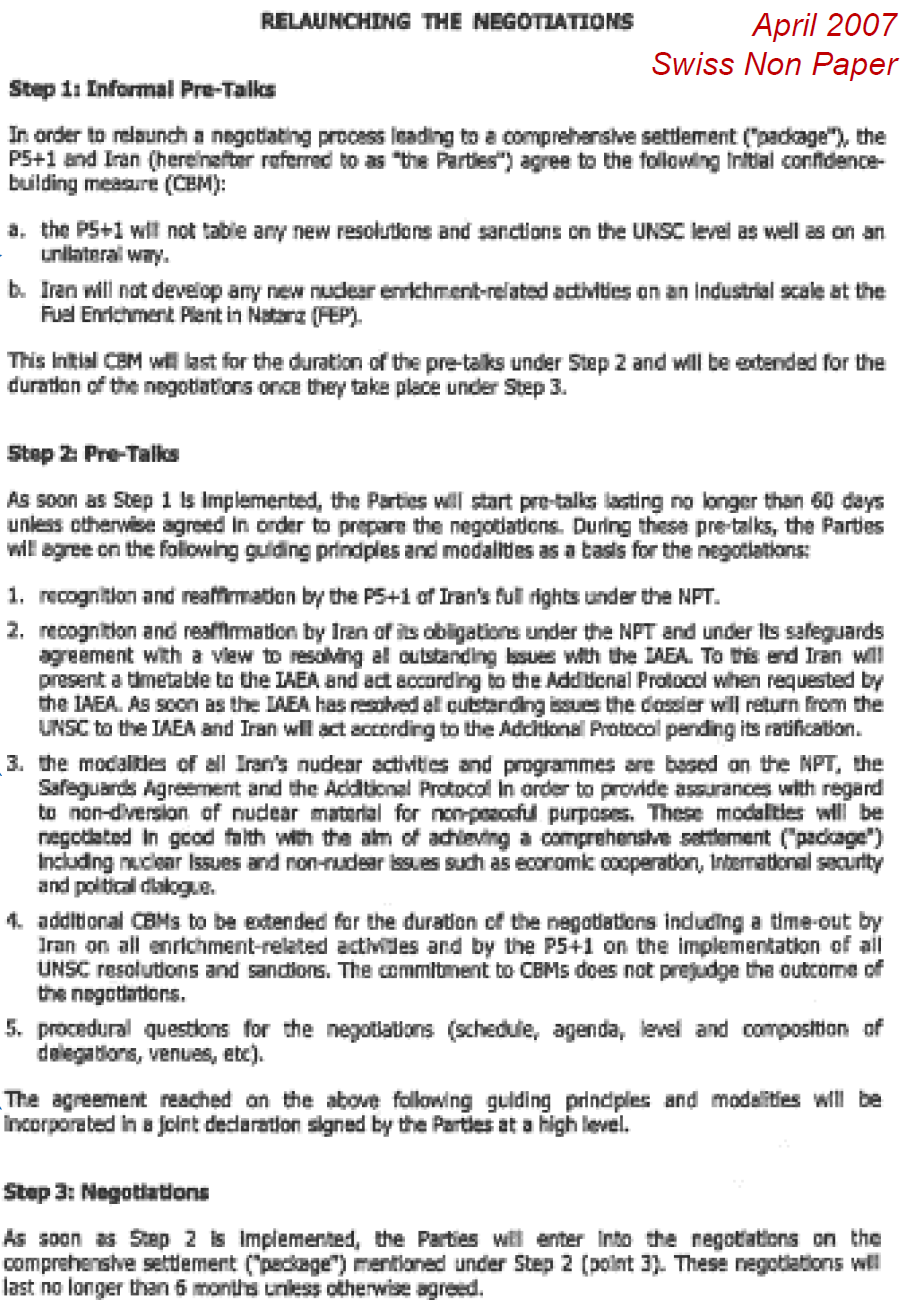
\includegraphics[width=\textwidth]{Pictures/Swiss_nonpaper.png}
\end{minipage}

\begin{figure}[H]
    \centering
    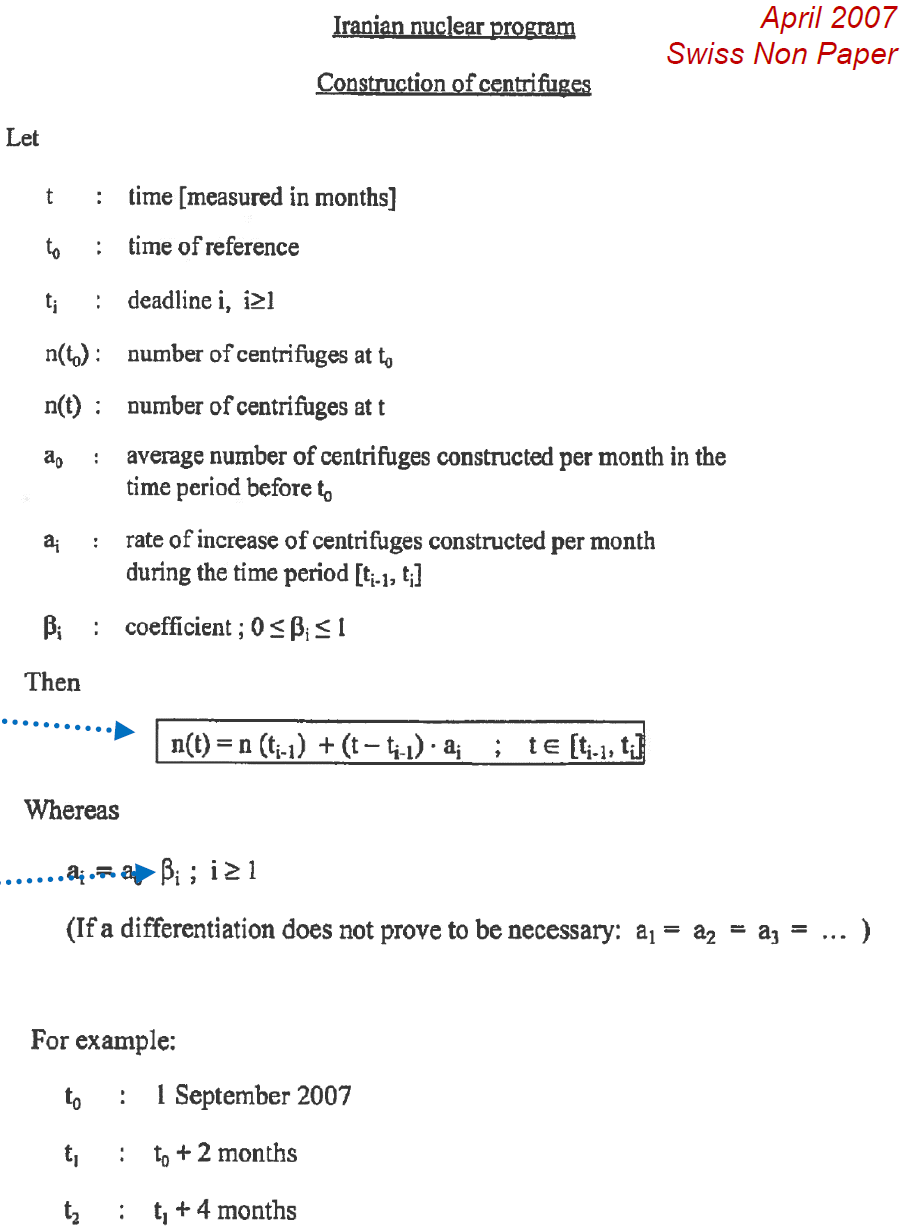
\includegraphics[width=0.5\textwidth]{Pictures/iran_nuclear_program_1.png}
    \hspace{5pt}
    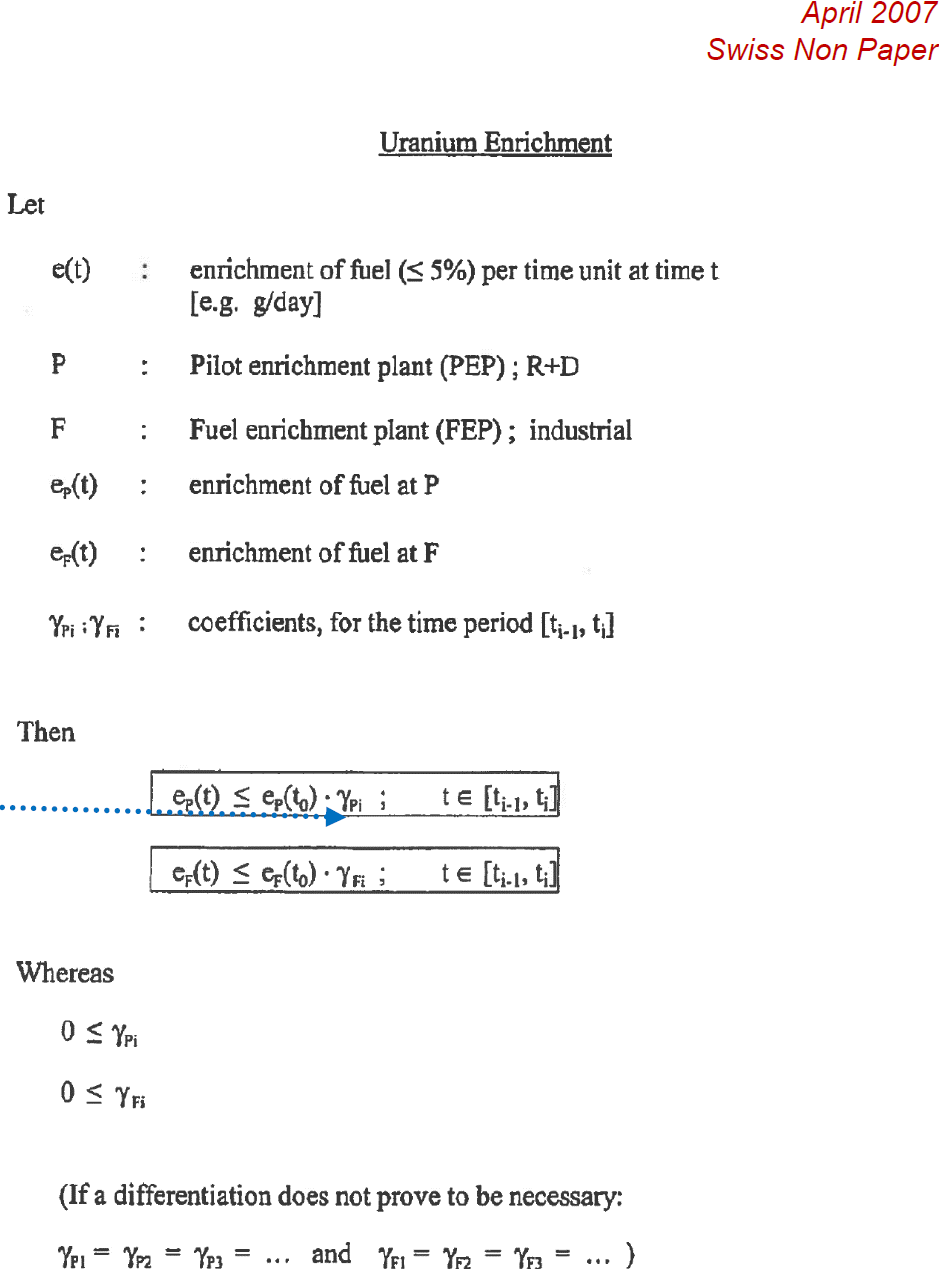
\includegraphics[width=0.47\textwidth]{Pictures/iran_nuclear_program_2.png}
\end{figure}

\paragraph{(d) Conclusions}

\begin{itemize}
    \item The parties could not agree to take up formal negotiations (until
        November 2013)
    \item Perhaps our math was too complicated (?), although
        Solana and Larijani (both mathematicians) understood it well
    \item However, this paper laid the basis for the first Geneva talks
        in July 2008. First high level meeting between US and IR since
        1980.
\end{itemize}

\paragraph{(e) Follow-up}

The two sides continued to:
\begin{itemize}
    \item increase the pressure via sanctions from $4$ to $\sim 80$
    \item increase the number of centrifuges from $\sim 200$ to
        $\sim 20'000$.
\end{itemize}
Game theoretical analysis:

\begin{figure}[h]
    \centering
    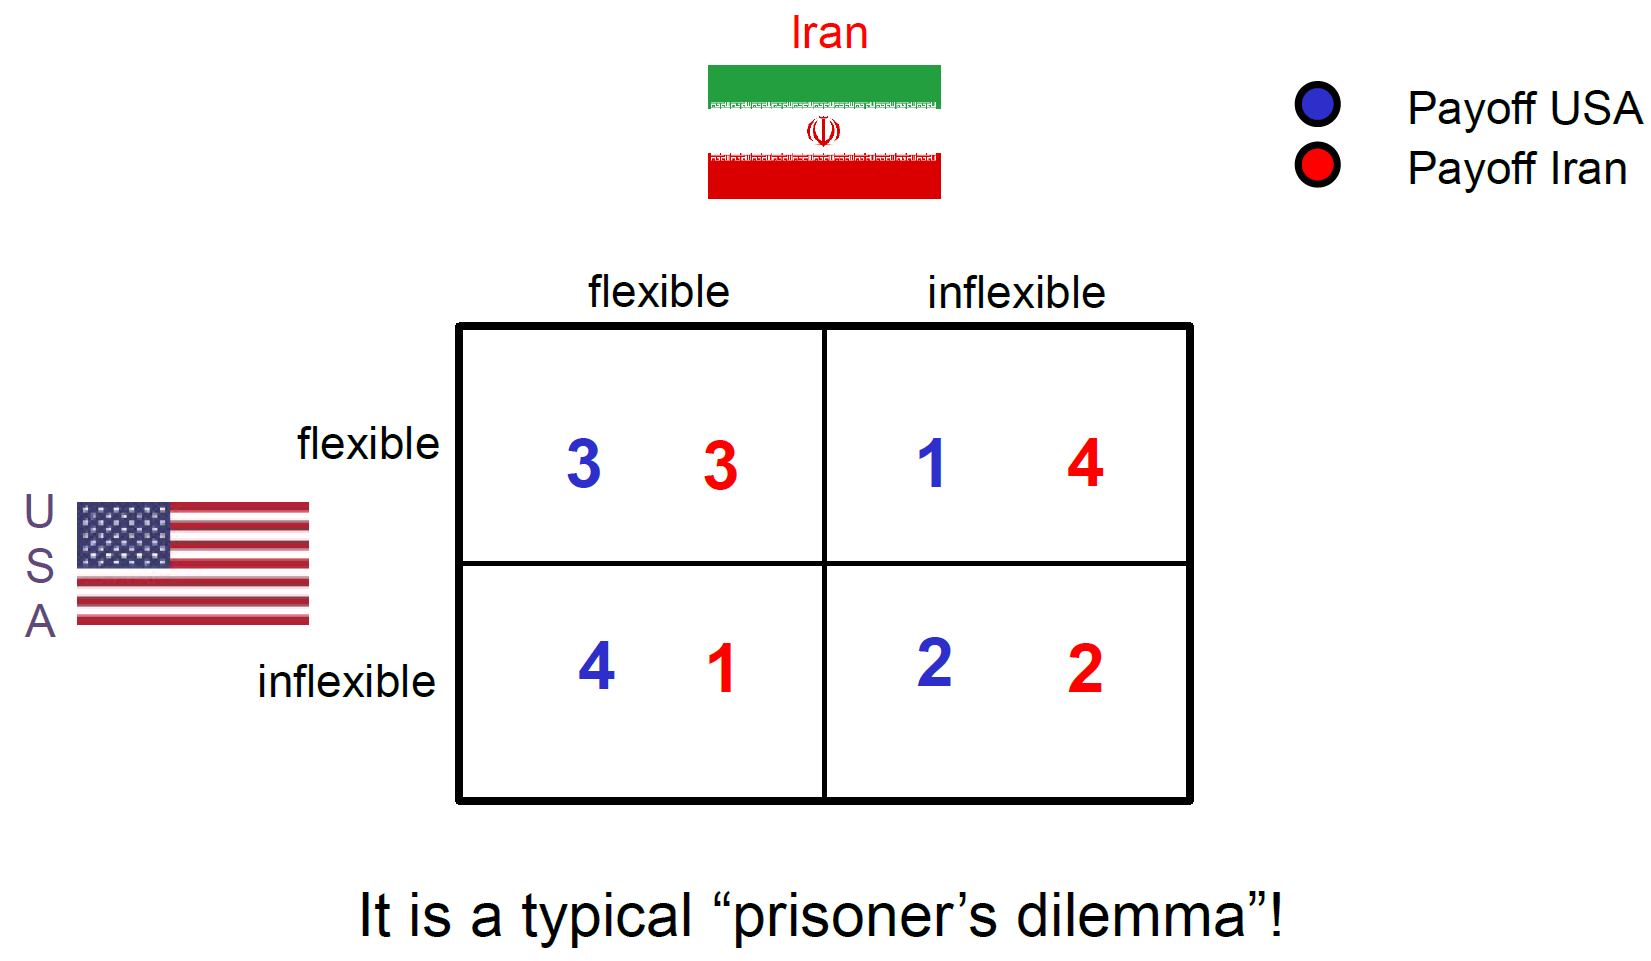
\includegraphics[width=0.47\textwidth]{Pictures/iran_us_game_theory_1.png}
    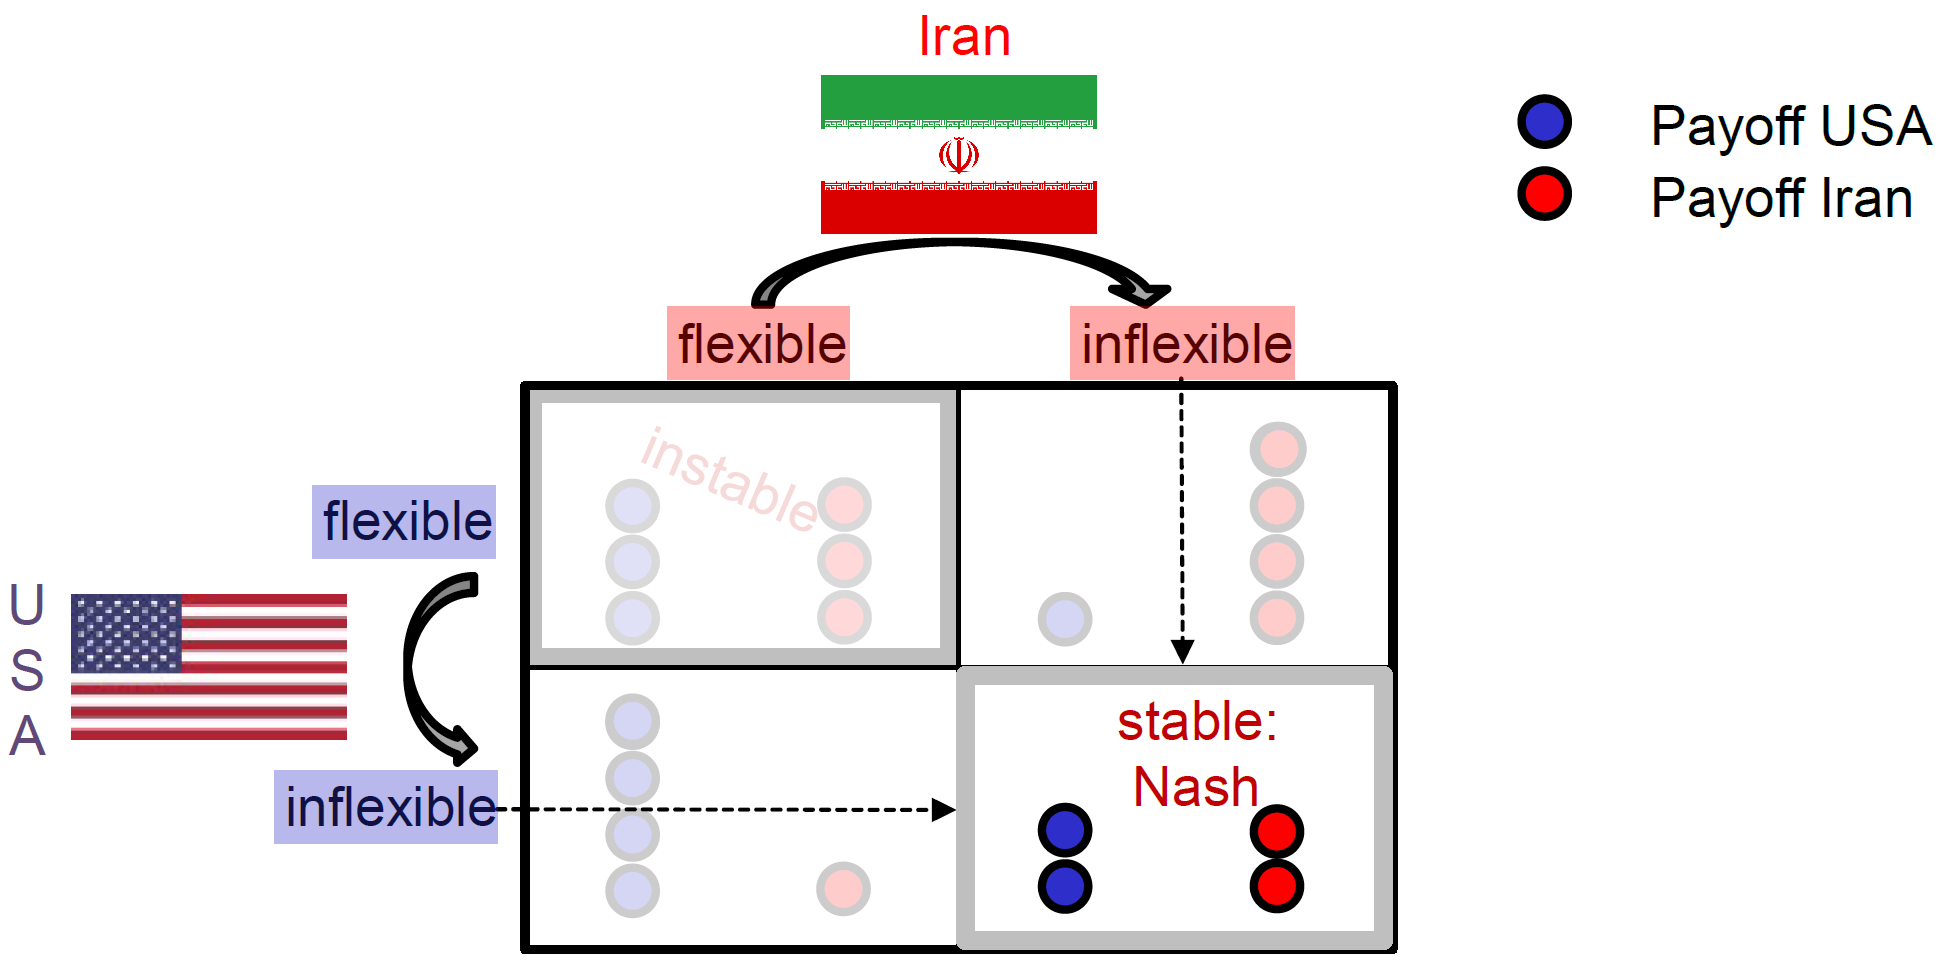
\includegraphics[width=0.52\textwidth]{Pictures/iran_us_game_theory_2.png}
\end{figure}

If both parties are flexible no negotiations occur and there is a lose-lose
situation. If one party increases its inflexibility, the other has to
increase as well to preserve the equilibrium (case of arms race).

Only when new elements appeared the situation changed: At the outset:
political changes in the governments: Bush to Obama and from
Mahmud Ahmadinedschad to Hassan Rohani.

Additionally, 4 new elements came to the forefront:

\begin{itemize}
    \item Sanctions started to hurt
    \item Enlargement of nuclear program problematic
    \item Iran's ambitions for regional power role
    \item Iran's Involvement in Syria crisis
\end{itemize}

\begin{figure}[h]
    \centering
    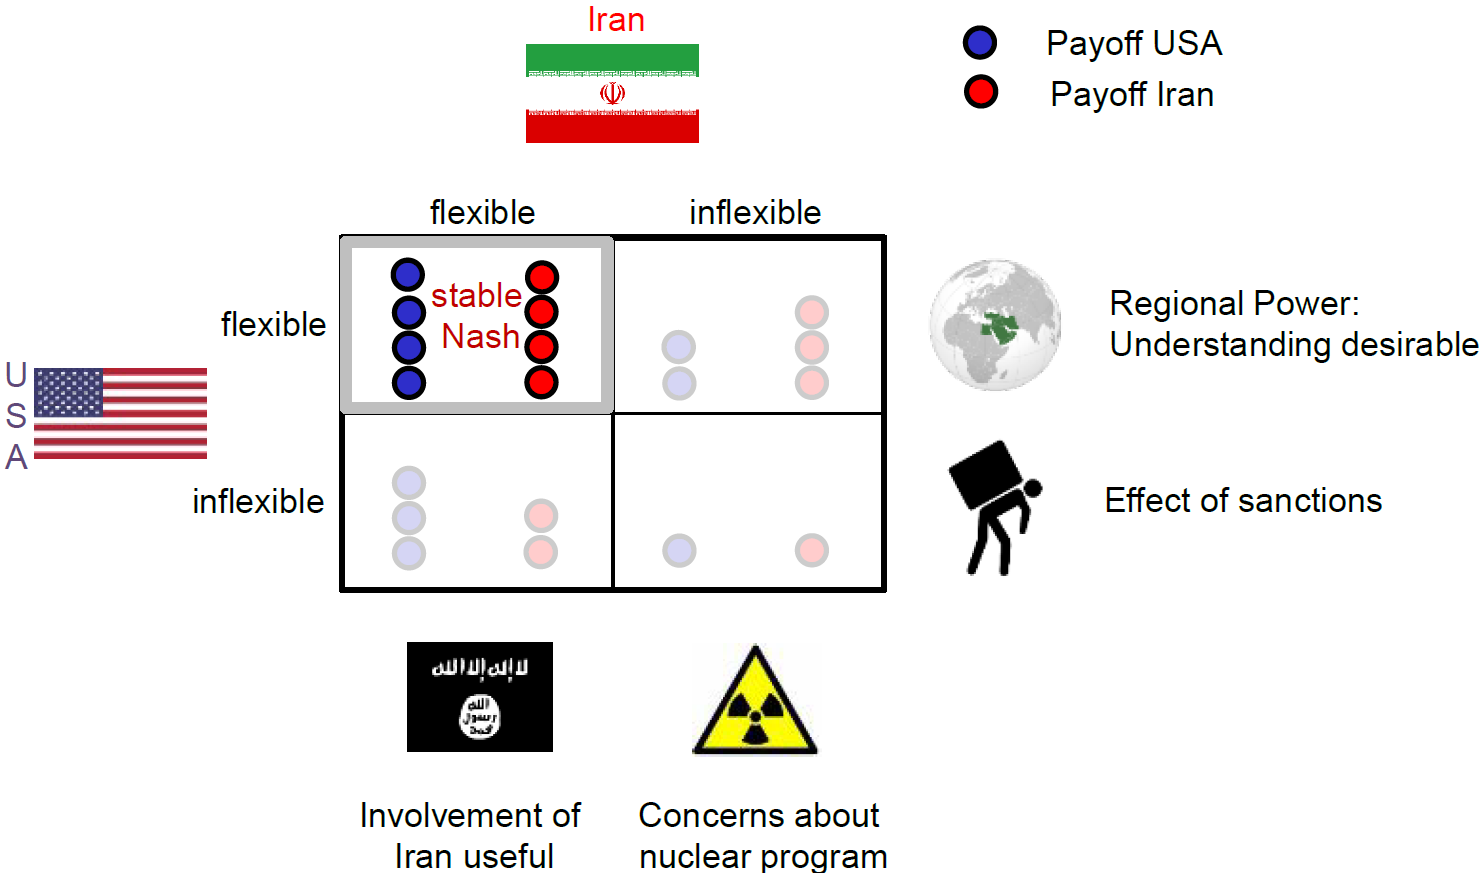
\includegraphics[width=0.5\textwidth]{Pictures/iran_us_new_game_theory.png}
    \caption{New allocation of payoffs after the new changes}
\end{figure}

As a result, it was no longer a "prisoner's dilemma" but a "concord" game.
The negotiations between P5+1 and Iran could start.

\begin{itemize}
    \item After the first Geneva-Talks (19.7.2008) a series of follow-up-meetings
        were held. With the above mentioned changes of the situation real negotiations
        started in fall 2013 and came to a (first) interim conclusion (Geneva interim
        agreement/"Joint Plan of Action"), signed on 24.11.2013.
    \item In these plan several of the Swiss proposal were taken up:
        \begin{itemize}
            \item no preconditions
            \item freeze-for-freeze
            \item phased approach
            \item negotiations [mainly] in Switzerland
        \end{itemize}
    \item This Plan of Action gave the framework for the following talks.
    \item The negotiations for a comprehensive/final agreement started on
        20.01.2014. Initially thought to last 6 months, they were prolonged
        until June 2015.
    \item On the 2.4.2015 they achieved an important (second) step towards the
        final agreement (to be finalized by end June 2015): "Parameters for a
        Joint Comprehensive Plan of Action" (Lausanne Agreement).
    \item On the 14.7.2015 the parties finally achieved the nuclear agreement
        in the "Joint Comprehensive Plan of Action" (JCPoA):
        \begin{itemize}
            \item Iran scaled back its nuclear program according to mutually
                agreed parameters
            \item The West conceded Iran's right of nuclear activities to a
                clearly defined degree, $\sim 6000$ centrifuges
            \item P5+1 lifted international sanctions in response
            \item Iran accepted long-lasting, robust verification by the IAEA
        \end{itemize}
    \item This agreement contributes to stability and peace in the Middle
        East and can be considered as a diplomatic success (of Obama [Kerry]
        and Rohani [Zarif]) and success of diplomacy.
    \item This Joint Plan of Actoin gave the framework for the following talks
        which resulted in the Vienna Agreement.
\end{itemize}

\paragraph{Development under Trump}

\begin{itemize}
    \item On 8.5.18 Trump withdraws from the Iran deal
        \begin{itemize}
            \item According to him, it was the "worst deal of all times"
            \item Trump is convinced that Iran didn't fulfil their part of
                the agreement
        \end{itemize}
    \item The US-sanctions against Iran were increased to a level above of
        what they were before the nuclear deal, seriously hurting the Iranian
        economy and putting the regime in a weak position.
    \item Due to pressure from the US, many international firms stopped
        dealing with Iran
        \begin{itemize}
            \item They had the choice between stop dealing with Iran
                or stop dealing with the US
        \end{itemize}
    \item Subsequently, tensions rose considerably, peaking at a US dronestrike
        killing Irani general Qasem Soleimani, for whose death Iran conducted
        retaliating missile strikes against US military bases in Iraq.
\end{itemize}

\paragraph{Back to cooperation under Biden?}

\begin{itemize}
    \item The situation is similar to the time before Obama
        \begin{itemize}
            \item The US want to contain the Iranian threat in the region
                globally
            \item Iran wants the US to ease off the sanctions
            \item Both want the other to move first (Chicken Game)
        \end{itemize}
    \item Political situation
        \begin{itemize}
            \item US Republicans (and some democrats) are not convinced the
                original deal was good
            \item Moderate Iranian president Rouhani, who will leave office
                in 2021, and current foreign minister Mohammed Javad Zarif,
                who was a key player during the negotiation of the 2015 deal,
                are under pressure from hardliners. Hardline-majority in the
                Iranian parliament wants to end negotiations completely.
            \item Potential backlash: Allied Israel and its newfound partners
                at the gulf don't want the US to deal with Iran
        \end{itemize}
\end{itemize}

\paragraph{Talks in Vienna}

\begin{itemize}
    \item A Joint Commission of the remaining participants to the Joint
        Comprehensive Plan of Action (JCPoA) met at the beginning of April
        2021 in Vienna to salvage the agreement.
    \item The US and Iran are joining for the second round of talks under the
        condition of Iran, that they will not directly engage with the US. The
        other participants - the UK, France, Germany, Russia, China and the EU
        - have thus to play the role of intermediaries, under the chairmanship
        of the EU.
    \item The delegations from Iranian and the US are residing in two separate
        hotels that are located 100m across the street from each other with the
        EU leading the shuttle diplomacy.
    \item While the talks are expected to go for months - and with recent attack
        on the Iranian nuclear facility looming - there is pressure to produce
        results before the presidential elections in Iran on 18 June 2021, where
        a hardliner could succeed the current centrist President Rouhani.
    \item There are also questions whether the 2015 deal is still as robust an
        agreement as it was then it was signed: in the past two years, Iran has
        developed new centrifuges that have altered the calculation on which
        the limits set by the 2015 deal was based.
\end{itemize}

\paragraph{Where do both sides stand?}

\begin{itemize}
    \item US positions
        \begin{itemize}
            \item Biden wants to re-join a deal, but it is not the number 1
                priority (Covid-Pandemic)
            \item US would prefer to negotiate a "longer and stronger" deal
            \item The US is willing to only lift those sanctions that are
                inconsistent with the JCPoA as part of a mutual return to
                compliance. This, however, does not necessarily include the
                sanctions imposed by the Trump administration on major Iranian
                entities under non-nuclear sanctions authorities (i.e. terrorism),
                which includes Iran's Central Bank and the National Iranian
                Oil Company. If these are not lifted it would be hard to imagine
                a benefit for Iran from a revival of the deal.
        \end{itemize}
    \item Iran Position
        \begin{itemize}
            \item Iran demands a lifting of all sanctions (even those that
                would be permissible under the deal, such as those on Iran's
                missile programme or relate to huma rights issues)
            \item Sanctions have to be lifted simultaneously and not in a
                step-by-step process. Iran would then verify their removal
                before bringing its nuclear programme back into compliance.
                Thus the question here: how much flexibility is there in Iran's
                position?
            \item Position will become tougher if a hardliner is elected President
                in June.
        \end{itemize}
\end{itemize}

\subsubsection{Deutsche Bahn (DB) train drivers' strike}
Conclict between Management and Labor Union

\paragraph{(a) Background}

\begin{itemize}
    \item DB has two trade unions:
        \begin{itemize}
            \item GDL (Gewerkschaft Deutscher Lokomotivführer) representing
                70\% of all DB employees
            \item EVG (Eisenbahn- und Verkehrsgesellschaft) representing majority
                of DB employees
        \end{itemize}
    \item Until July 2014, the tasks of the two trade unions were clearly distributed
        \begin{itemize}
            \item GDL negotiates working conditions for train drivers
            \item EVG negotiates working conditions for all other DB workers
        \end{itemize}
    \item Wage negotiations in July 2014: GDL wanted negotiations in the name
        of train crew (train conductors etc.) as well, while EVG wanted to
        negotiate in the name of all DB employees.
    \item Train drivers followed the call of GDL and stopped working several
        times between September 2014 and May 2015.
\end{itemize}

\paragraph{(b) Negotiations}

Conflict between GDL and DB

\begin{itemize}
    \item GDL demands:
        \begin{itemize}
            \item 5\% pay increase
            \item Workweek reduces from 39 to 37 hours
            \item To negotiate for all? (negotiate on behalf of 17'000 train
                stewards) DB employees
        \end{itemize}
    \item DB offered:
        \begin{itemize}
            \item Raise pay of train drivers by 5\% for 30 months
            \item Hire 200 more train drivers to allow for more flexible
                working times
        \end{itemize}
    \item Strike of November 2014:
        \begin{itemize}
            \item On 5 November DB offered to go to mediation/arbitration, GDL refused
            \item On 6 November DB filed an injunction with the labor court in Frankfurt
            \item Court decided the strike is legal
            \item GDL finished the strike one day earlier as a "gesture of good will"
        \end{itemize}
\end{itemize}

Conflict between unions GDL and EVG
\begin{itemize}
    \item Struggle for influence between GDL and EVG
    \item DB could negotiate different vollective agreements with each of the
        groups
    \item EVG offered that the majority union negotiates deals $\rightarrow$
        GDL negotiates train drivers conditions and EVG negotiates continuations
        for all other DB workers. GDL refused this offer.
    \item Act of collective agreement plans that only the collective agreement
        of the union with the most members does apply.
\end{itemize}

There was a huge criticism of the strike. The costs were also really large,
be it for the DB or the passengers.

\vspace{1\baselineskip}

Assesment
\begin{itemize}
    \item Germany's internal legal difficulties about the question who represent
        the workers (only the main union or also the competing unions)
    \item Probably, also a person's driven strike
    \item Mr. Claus Weselsky (GDL) is perceived as tough trade union leader
    \item Difficult to give good advice for avoiding strikes, however it is
        always important for the management to cultivate good relations with
        the trade union.
\end{itemize}

\paragraph{(c) (Possible) Results}

Conflict between Management and Labor Union:

\vspace{1\baselineskip}

Concept
\begin{itemize}
    \item Often conflicts between the management and labor union involve many
        issues
    \item To facilitate win-win process, a good preparation is useful:
        \begin{itemize}
            \item Prepare a list of all issues
            \item For each issue: What resolutions are possible for this issue?
            \item Distribute points which represent your preferences over issues
                and resolutions levels
            \item Anticipate points distribution over the issues and resolutions
                levels from your counterpart's point of view
            \item $\rightarrow$ These preparation steps are the basis for so
                called 'additive scoring system'
        \end{itemize}
\end{itemize}

\begin{figure}[H]
    \centering
    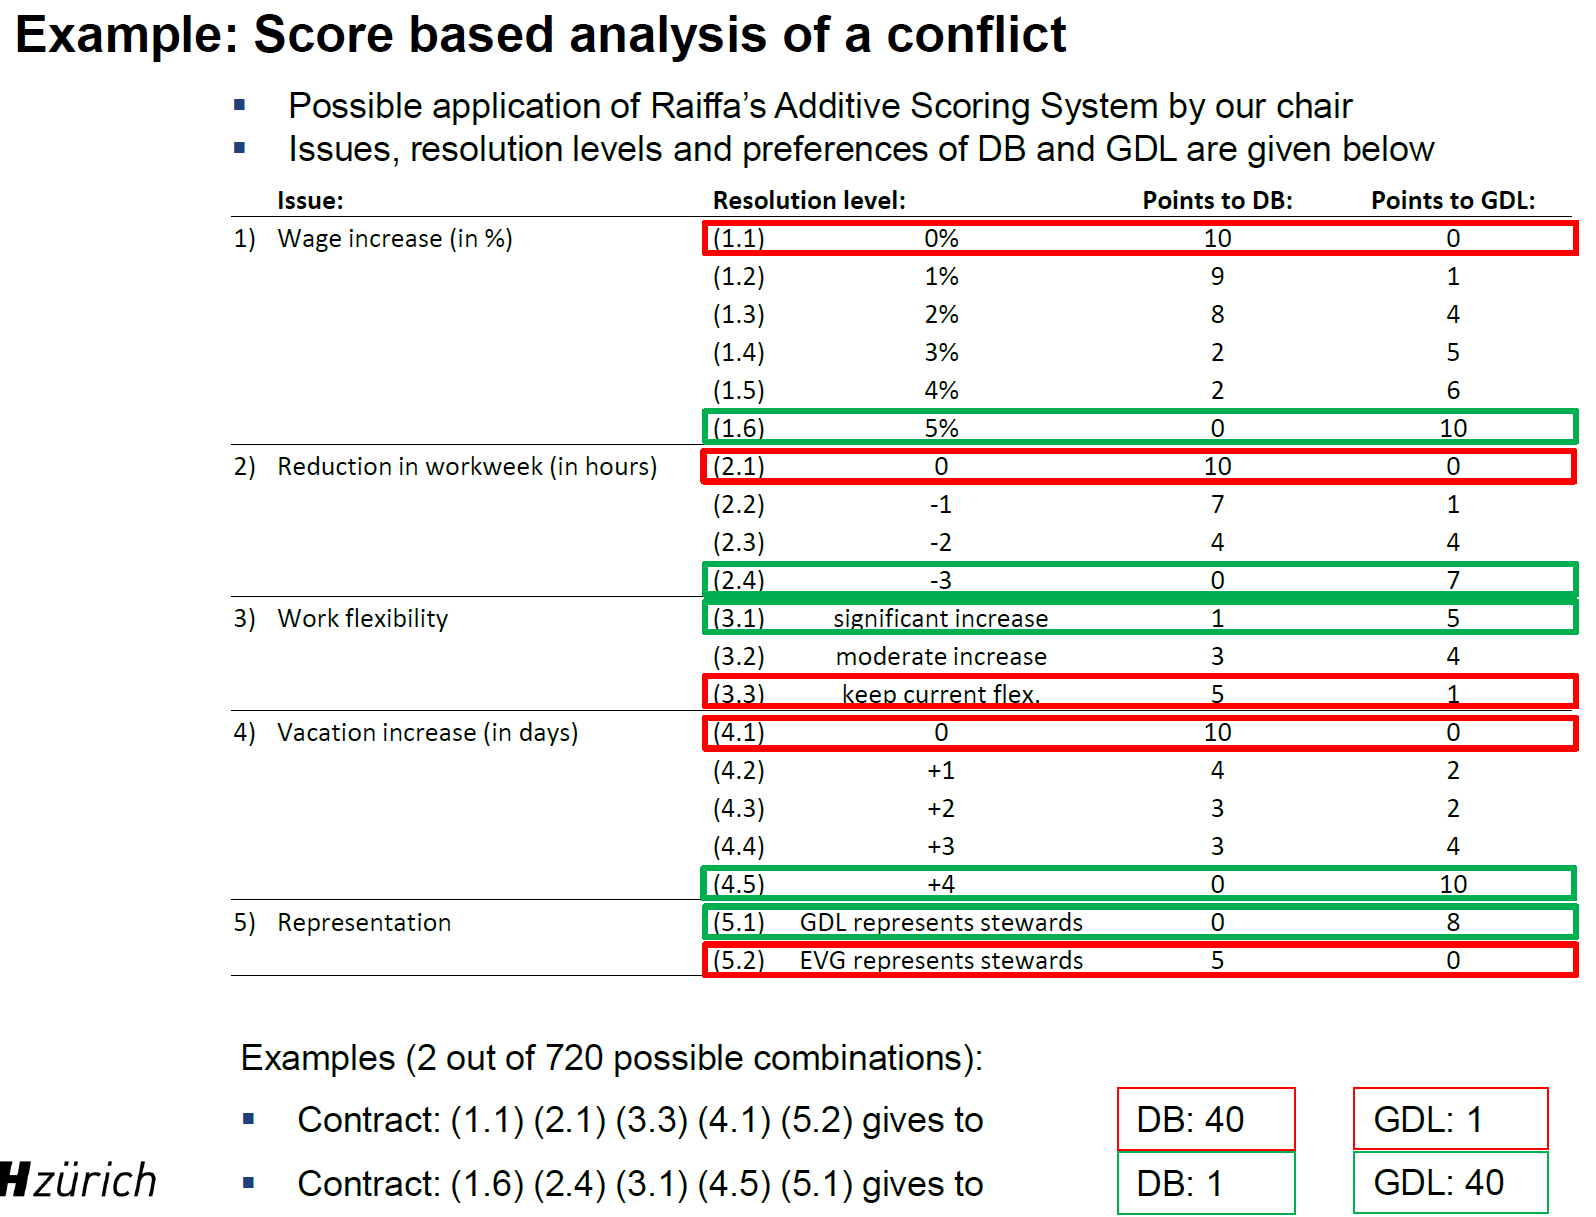
\includegraphics[width=0.48\textwidth]{Pictures/Score_based_analysis_DB.png}
    \hspace{5pt}
    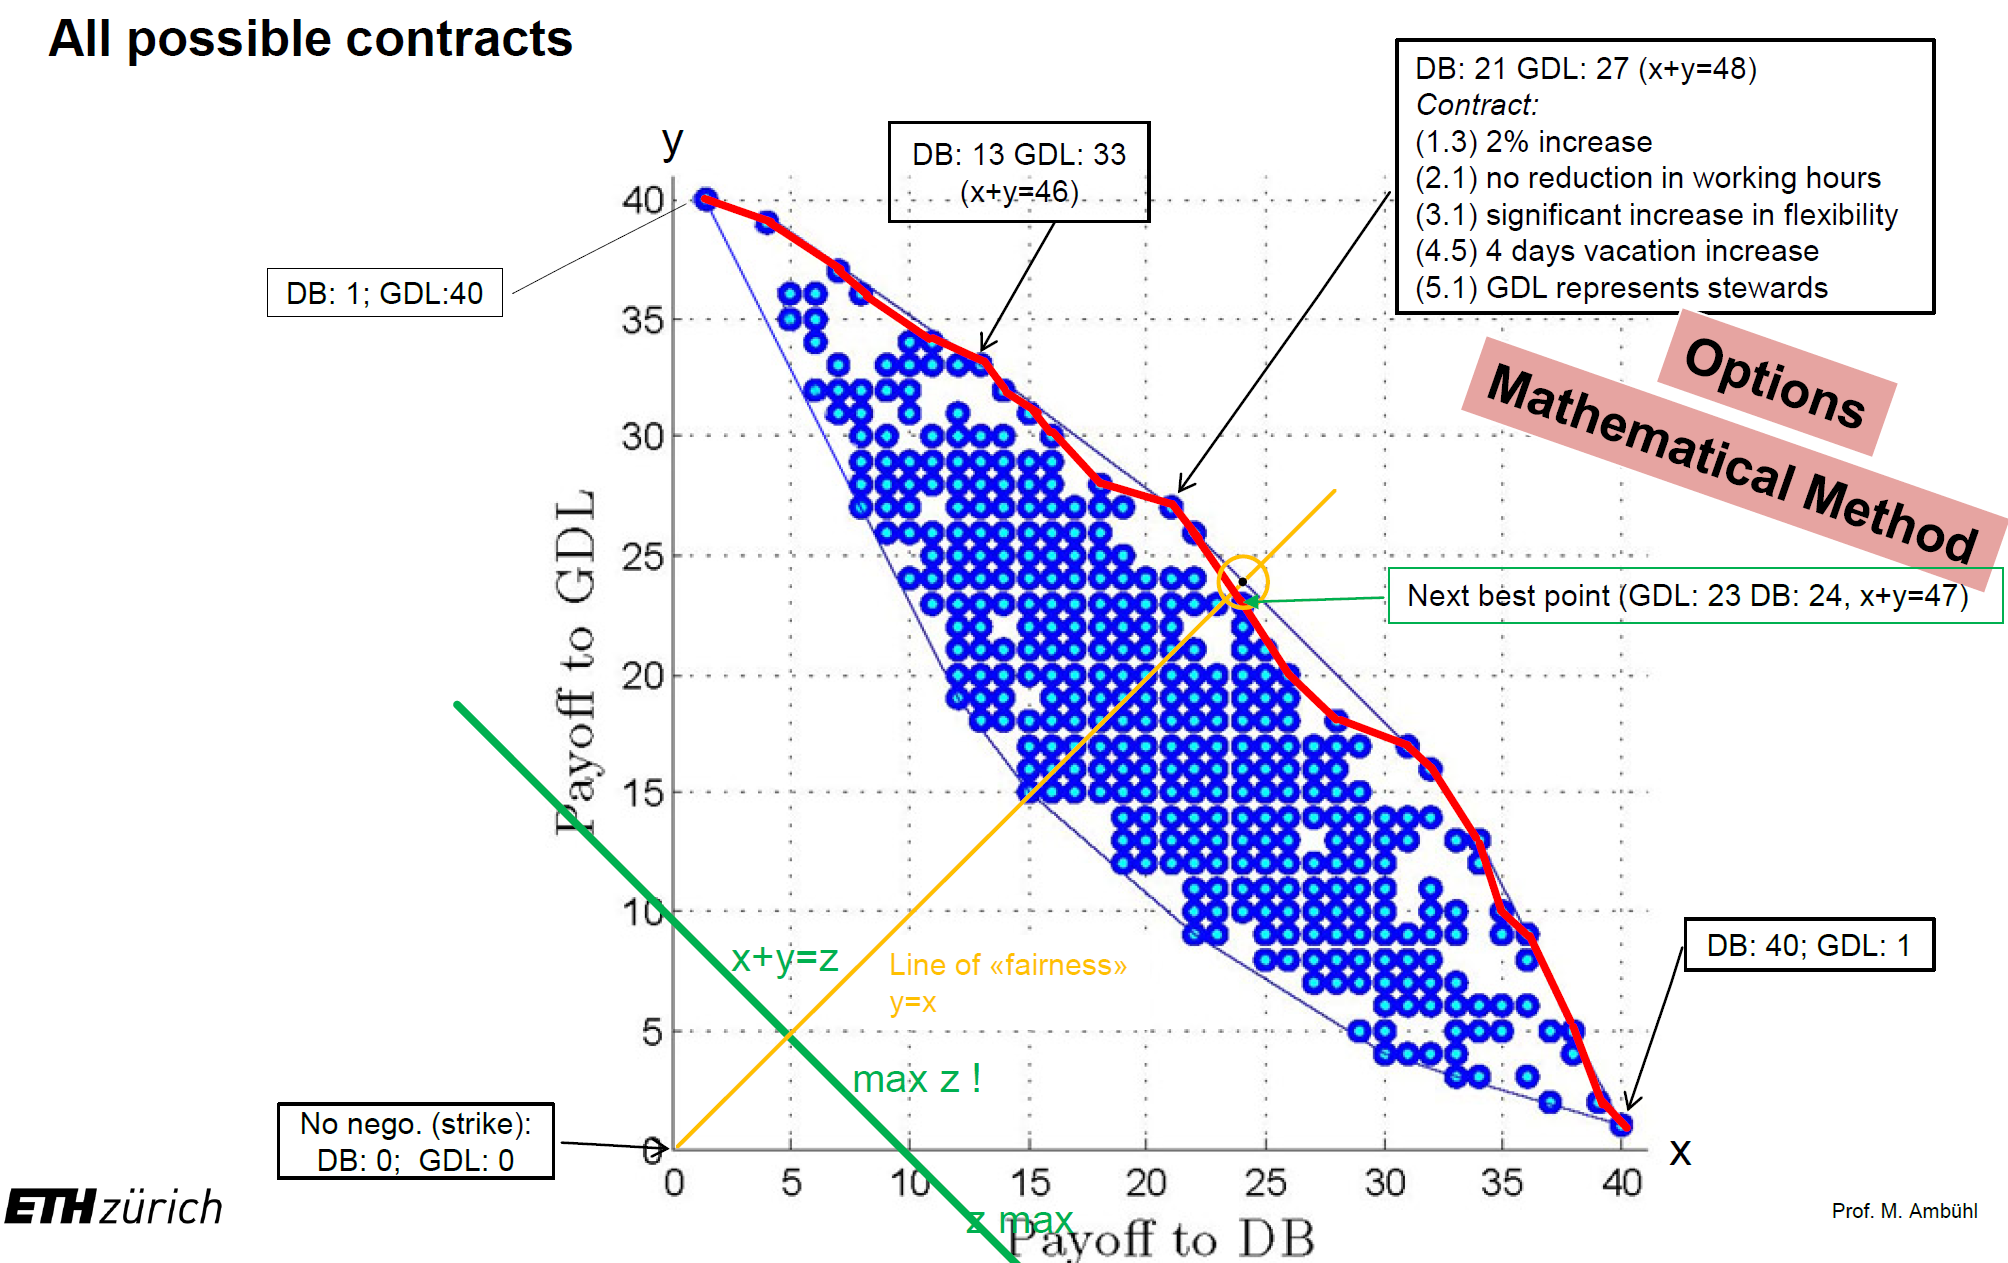
\includegraphics[width=0.48\textwidth]{Pictures/Possible_solutions_DB.png}
\end{figure}

What are the potential weaknesses of the score-based conflict analysis approach?
\begin{itemize}
    \item Structuring the issues
    \item Assigning payoffs
    \item Avoiding tactical scoring
    \item Concerning the scoring:
        \begin{itemize}
            \item Standardizing the metrics
            \item Ensuring same end-points
            \item Ensuring distribution
        \end{itemize}
\end{itemize}

\paragraph{(d) Comments}
\begin{itemize}
    \item 'Quantification' of the problem may help
        \begin{itemize}
            \item to structure the problem
            \item to understand possible tradeoffs
        \end{itemize}
    \item For mediator: Look for contracts in the 'north-east' direction
    \item Trust is crucial: Mediator can propose an optimal contract on Pareto
        frontier only if he has the true preferences of the parties (i.e.
        if they do not manipulate the values of certain outcome)
    \item Weselsky refuses to appeal a mediator: "Wir lassen nicht über
        Grundrechte schlichten"
\end{itemize}
